
\chapter{MODELOS MATEMÁTICOS Y SIMULACIÓN}

%Contadores y formato para numeracion de elementos
\renewcommand{\thefootnote}{\arabic{footnote}}
\renewcommand{\theequation}{\arabic{chapter}-\arabic{equation}}
\renewcommand{\thefigure}{\arabic{chapter}.\arabic{figure}}
\renewcommand{\figurename}{Figura}
\renewcommand{\tablename}{\textbf{Tabla}}
\renewcommand{\thetable}{\textbf{\arabic{chapter}-\arabic{table}}}
\newcounter{definitionN}
\newcounter{exampleN}
\newcounter{tableN}
\newcounter{footN}
\newcounter{algorithmN}
\stepcounter{definitionN}
\stepcounter{exampleN}
\stepcounter{tableN}
\stepcounter{footN}
\stepcounter{algorithmN}
\bibliographystyle{apalike}

%Diana Carolina Guarin Angulo
\newpage
En este capítulo se desarrollan las ideas de \textit{\textbf{Sistema, Modelo}} (matemático) y \textit{\textbf{Solución del modelo}}.

Dentro de estos conceptos se plantea el modelo \textbf{SAO} (\textbf{S}istema, \textbf{A}mbiente, \textbf{O}bservatorio), descrito con más detalles en \cite{trivino2010complexSystems} sobre el cual se estructura el estudio formal de un \textbf{Sistema} (complejo) \textbf{S}.

\section{INTRODUCCIÓN}\label{sec:intro}
\setcounter{equation}{0}

La realidad, en medio de la cual se encuentran las personas y los objetos que posibilitan su supervivencia en un mundo generalmente hostil, es compleja. Que una persona pueda sobrevivir en un entorno complejo es gracias, en parte, a la capacidad de abstracción con la que cuentan los humanos (y en general los seres vivos). La abstracción permite representar internamente la realidad a través de esos factores que son esenciales y suprimir los detalles (seguramente importantes) pero innecesarios en un momento particular. Reducir esa realidad a lo relevante le posibilita a las personas comprender lo importante del entorno y le da la capacidad de adoptar decisiones con relativa \textit{eficiencia} pero eso sí, principalmente, con una alta \textit{eficacia}.\\

En este contexto, se llamará \textbf{\textit{Sistema}} a un trozo de la realidad que tiene algún fin particular, el \textbf{\textit{Ambiente}}, que también es un pedazo de la realidad, brinda las condiciones necesarias (y al menos suficientes) para que, en el caso de que el sistema se encuentre inmerso en él, pueda actuar en la búsqueda del cumplimiento de su objetivo.\\

Los humanos, a través de la \textit{ciencia}, han construido algunos sistemas particulares (que como tales son piezas de la misma \textit{realidad}) cuya finalidad es servir de herramientas que permiten comprender la \textit{naturaleza de la realidad} a través de la acción de sistemas en ciertos entornos pero, en particular, comprender el éxito o el fracaso de un sistema en un ambiente. Para ello evalúan el desempeño del sistema en estudio en medio de un ambiente particular. Cada uno de esos sistemas especializados en medir el comportamiento del sistema actuando en un ambiente se les denomina \textbf{\textit{Observatorio}}.\\

A esa abstracción de la realidad que realizan en su permanente quehacer tanto el sistema como el observatorio se denomina \textbf{\textit{modelo}} (de la realidad) pero nótese que el modelo del sistema no tiene por qué ser el mismo del observatorio ni mucho menos de la misma naturaleza. Con frecuencia, el modelo es de naturaleza matemática, caso en el cual corresponde a un conjunto de ecuaciones. A la determinación de los niveles de las variables que resuelven el sistema de ecuaciones se le conoce como la \textbf{\textit{solución del modelo}} matemático.\\

El propósito de este capítulo es, por lo tanto, estudiar los conceptos de \textbf{\textit{Sistema, modelo}}  y \textbf{\textit{solución del modelo}}  y su rol dentro del campo de los modelos estocásticos en computación.

\section{VARIABLE TRASCENDENTAL: EL ESPACIO-TIEMPO}\label{sec:varTrasc}

\textbf{Definición \arabic{chapter}-\arabic{definitionN}: Naturaleza}\\

\stepcounter{definitionN}
Conjunto de todo lo que \textit{\textbf{existe}}, se rige y se armoniza a través de sus propias leyes. Una armonía entendida como la proporción y correspondencia de los objetos (físicos o abstractos) que componen el todo y que hace que ellos no discuerden o se rechacen principalmente (pero no únicamente) cuando simultáneamente concurren en la consecución de algún fin.\\

El sistema y el modelo general se describen formalmente mediante \textit{\textbf{variables}}, \textit{\textbf{parámetros}} y \textit{\textbf{funciones}} que describen características y representan comportamientos. La naturaleza y, en tal virtud, el ambiente está caracterizada por sus variables de estado denominadas \textit{\textbf{El Tiempo— Espacio}}.\\ 

\textbf{Ejemplo \arabic{chapter}-\arabic{exampleN}: El universo \textfrak{U}}\\

\stepcounter{exampleN}
El universo físico que conocemos conformado por las \textit{galaxias}, las \textit{estrellas}, los \textit{planetas} y todos los \textit{cuerpos celestes} regidos y “armonizados” por un conjunto de leyes, entre ellas la ley de la gravitación universal, que generan un orden o \textit{cosmos} que llamamos \textit{mundo} es, probablemente, el
caso más representativo de \textit{naturaleza}.\\

\textbf{Ejemplo \arabic{chapter}-\arabic{exampleN}: Red de computadores estocástica y dinámica}\\

\stepcounter{exampleN}
El mundo digital generado al interior de un sistema de redes de computadores (dispositivos) conectados a través de canales inalámbricos de forma dinámica y estocástica con el fin de brindar servicios de cómputo mediante abstracciones tales como las de agentes artificiales y comunidades de agentes artificiales que cooperan con el propósito de brindar “servicios” al sistema de red es una obra de ingeniería que cumple con rigor la Definición \arabic{chapter}-1 y, en consecuencia, relativo a la
disciplina de la computación es \textit{naturaleza}.\\

\textbf{Definición \arabic{chapter}-\arabic{definitionN}: Espacio-Tiempo}\\

\stepcounter{definitionN}

El Espacio─Tiempo es un espacio vectorial\footnote[\arabic{footN}]{Matemáticamente un \textit{\textbf{espacio vectorial}} sobre un campo $K$ es un conjunto $T \neq \varnothing$ dotado de dos operaciones para las cuales será cerrado: 1.) Operación interna de Suma \textit{\begin{matrix} $+:$ & $TxT$ &$\to$& $T$ \\ \ & $(t_1,t_2)$ & \to & $+(t_1,t_2)$ \end{matrix}} con las propiedades conmutativa, asociativa, elemento neutro \textbf{$e$} y elemento opuesto \textbf{$-t$}. 2.) Operación externa producto \textit{\begin{matrix} $\bullet:$ & $KxT$ &$\to$& $T$ \\ \ & $(t_1,t_2)$ & \to & $\bullet(t_1,t_2)$ \end{matrix}} con las propiedades asociativa, distributiva del producto con respecto a la suma de vectores y distributiva con respecto de la suma de escalares.} $T \in \mathbb{R}^m$, o equivalentemente $T=(T_1,T_2,...,T_m)$, mediante el cual los \textit{objetos} de la \textit{naturaleza} pueden ser ubicados en las coordenadas $t=(t_1,t_2,...,t_m)$ en un universo particular.\\

\stepcounter{footN}
En la Definición \arabic{chapter}-2 el parámetro \textit{m} representa la dimensión espacio-temporal de la naturaleza. Es frecuente que $m=4$ y que $T_1: tiempo$ como se ilustra en la Figura \arabic{chapter}.1. Es decir, que un objeto o entidad se ubica dentro de ese entorno en cuatro (4) dimensiones. La primera de ellas el tiempo en sentido cronológico y las restantes tres (3) corresponden a la ubicación espacial tal como la conocemos y manejamos en nuestra realidad (\textit{\textbf{altura, anchura, profundidad}}). Sin embargo, a decisión y conveniencia del diseñador del sistema o modelo pueden emplearse más o menos dimensiones.\\

En el caso del universo físico conocido es frecuente (pero no universalmente aceptado) adoptar el espacio métrico euclidiano $(T,d)$ donde $T$ es un espacio vectorial euclidiano (es decir, donde se cumplen los cinco postulados de Euclides) y sobre el cual se asocia la medida de \textit{distancia} entre dos puntos $T^{(1)}, T^{(2)}  \in \mathbb{R}^m $ dada por la expresión \ref{twoPointDist}.\\

\begin{equation}
d(T^{(1)},T^{(2)})=\parallel T^{(1)}-T^{(2)} \parallel = \sqrt{\sum^{m}_{i=1}(t_i^{(1)}-t_i^{(2)})^2}
\label{twoPointDist}
\end{equation}

De acuerdo con la Figura \arabic{chapter}.1 un objeto (por ejemplo un agente artificial) puede ubicarse en un instante cronológico en algún punto del espacio tridimensional. A menos que se diga lo contrario, la variable trascendente Espacio-Tiempo será considerada tetra-dimensional con la interpretación aquí señalada.\\
\begin{figure}[H]
     \begin{center}
         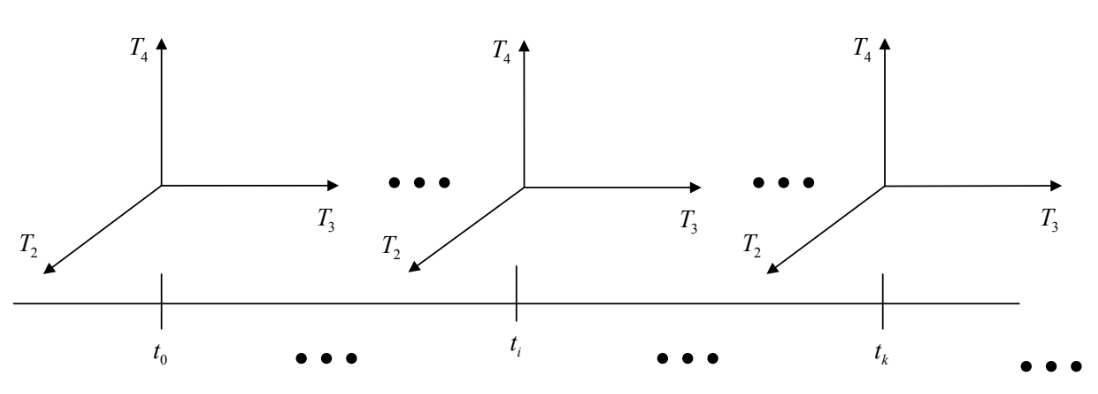
\includegraphics[width=120mm]{chapters/chapter4/figures/espacioTiempo.png}
     \end{center}
     \textbf{\caption{El espacio tiempo tridimensional y tiempo cronológico}}
     \label{fig:1}
\end{figure}

\section{SISTEMA Y AMBIENTE}\label{sec:sistAmbiente}
\textbf{Definición \arabic{chapter}-\arabic{definitionN}: Sistema $\mathbb{S}$}\\

\stepcounter{definitionN}
De acuerdo con \cite{klir2006uncertainityInfoTheory} un sistema $\mathbb{S}$ es un conjunto de entidades o elementos que se interrelacionan entre sí para cumplir uno o más objetivos.\\

\textbf{Ejemplo \arabic{chapter}-\arabic{exampleN}: Pozo Petrolero}\\

\stepcounter{exampleN}

Un pozo petrolero $\mathbb{S}$ es un ingenio humano creado con el fin de poner en contacto un yacimiento de hidrocarburos con la superficie. Dicha conexión entre el yacimiento y la superficie, se realiza con perforaciones de diferentes diámetros llevada a cabo por un taladro capaz de manipular barrenas (usualmente de acero) con rosca en espiral, para la extracción del crudo o gas. Al cumplir la Definición \arabic{chapter}—3, esta obra de ingeniería $\mathbb{S}$ es un sistema.\\

En este caso, los (principales) elementos del sistema son el \textit{hidrocarburo}, el \textit{yacimiento}, el \textit{conjunto de ductos}, los \textit{aparatos} que posibilitan la extracción, las \textit{personas} que operan el pozo, etc. Por otro lado, son claras algunas relaciones que saltan a la vista entre ellos: la relación de “contener” sostenida entre el yacimiento y el crudo, la relación de “extraer” sostenida entre el conjunto de ductos y la maquinaria de extracción, la relación de “operar” presente entre las personas y las máquinas, entre muchas otras relaciones posibles.\\

\textbf{Ejemplo \arabic{chapter}-\arabic{exampleN}: Dispositivo electrónico de suma binaria.}\\

\stepcounter{exampleN}

Un sumador binario en serie es un sistema $\mathbb{S}$ que se puede usar para obtener el resultado de la operación $x+y$. Sean $x=x_5x_4x_3x_2x_1 = 00111$ y $y=y_5y_4y_3y_2y_1 = 01101$ dos números binarios donde $x_1$ y $y_1$ son los bits menos significativos. Los primeros ceros de $x$ y $y$ están ahí para hacer que las cadenas tengan la misma longitud y para garantizar suficientes lugares para completar la suma. La Figura \arabic{chapter}.2 esquematiza esa operación matemática donde $z=z_5z_4z_3z_2z_1 $ es el resultado de la suma y, al igual que con los sumandos, tiene el bit menos significativo en $z_1$.\\

\begin{figure}[H]
     \begin{center}
         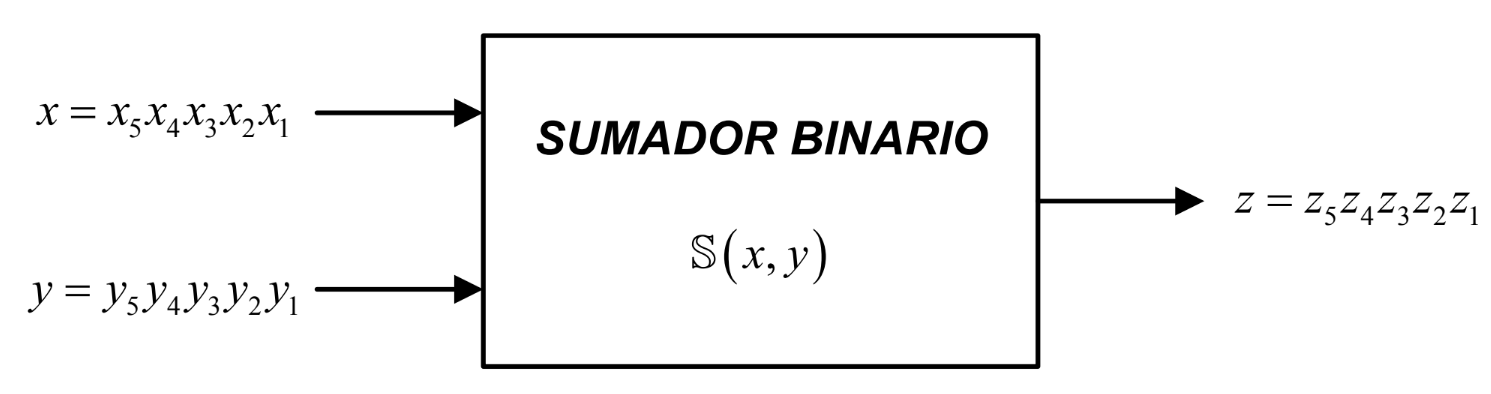
\includegraphics[width=120mm]{chapters/chapter4/figures/sumadorBinario.png}
     \end{center}
     \textbf{\caption{Dispositivo electrónico que suma dos números binarios.}}
\end{figure}

\textbf{Ejemplo \arabic{chapter}-\arabic{exampleN}: Máquina expendedora de chocolatinas.}\\

\stepcounter{exampleN}

Supóngase que en la Facultad de Ingeniería, una máquina $\mathbb{S}$ expendedora de golosinas dispensa dos sabores de chocolatinas: Chocolate negro $(CN)$ y Chocolate blanco $(CB)$. El costo de una unidad de cualquiera de los dos sabores es de $\$200$. La máquina acepta monedas de $ \$50, \$100, \$200 $ y devuelve el cambio necesario.\\

Un día Luis, un estudiante de Modelos estocásticos, decide que le gustaría una Chocolatina negra. Él va a la máquina expendedora, inserta dos monedas de $ \$50 $ y una moneda de $\$100$, en ese orden, y presiona el botón negro, denotado $(BN)$. Paso seguido la máquina le suministra la chocolatina negra. (Para obtener una de chocolatina blanca se presiona el botón blanco, que se denomina $(B)$\\

\begin{table}[h]
\centering
\begin{tabular}{|l|l|l|l|l|l|}
                 & \multicolumn{1}{c|}{$t_0$} & \multicolumn{1}{c|}{$t_1$} &\multicolumn{1}{c|}{$ t_2$} &\multicolumn{1}{c|}{ $t_3$}&\multicolumn{1}{c|}{ $t_4$}\\ 
                 \hline
\textbf{Estado}  & (1) $q_0(\$0)$ & (4) $q_1(\$50)$ & (7) $q_3(\$100)$ & (10) $q_4(\$200)$ & (13) $q_0$ \\ \hline
\textbf{Entrada} & (2) $\$50$ & (5) $\$50$ & (8) $\$100$ & (11) $(BN)$ &  \\ \hline
\textbf{Salida}  & (3) Nada & (6) Nada & (9) Nada & (12) $(CN)$ &  \\ 
\end{tabular}
\caption{\textbf{Secuencia de eventos en la compra de Luis.}}
\label{tab:compraLuis}
\end{table}
\stepcounter{tableN}

El procedimiento seguido por Luis, al hacer su compra, puede representarse como se muestra en la Tabla ~\ref{tab:compraLuis} donde $t_0$ es el tiempo inicial, cuando él inserta su primera moneda, y $t_1$, $t_2$, $t_3$, $t_4$, son momentos posteriores en el tiempo, con $t_1 < t_2 < t_3 < t_4$. Los números $(1),(2),(3),...,(13)$ en esa tabla indican el orden de los \textit{\textbf{eventos}} (para una definición más detallada de este concepto, véase la Definición \arabic{chapter}—12 ) en la compra de la chocolatina negra. Para cada entrada en el tiempo $t_i$, $0\leq i \leq 3$, hay en ese momento una salida correspondiente y luego un cambio de estado. El nuevo estado en el tiempo $t_{i+1}$ depende tanto de la entrada como del estado (presente) en el tiempo $t_i$. La Tabla ~\ref{tab:compraAmigoLuis} muestra la secuencia de eventos en otra compra de chocolatina que realiza un amigo de Luis.\\

\begin{table}[H]
\centering
\begin{tabular}{|l|l|l|l|}
                 & \multicolumn{1}{c|}{$t_0$} & \multicolumn{1}{c|}{$t_1$} &\multicolumn{1}{c|}{$ t_2$} \\ \hline
\textbf{Estado}  & (1) $q_0(\$0)$ & (4) $q_4(\$200)$ & (7) $q_0$   \\ \hline
\textbf{Entrada} & (2) $\$500$ & (5) $(B)$ &    \\ \hline
\textbf{Salida}  & (3) $\$300$ de cambio & (6) $CB$ &   \\ 
\end{tabular}
\caption{\textbf{Secuencia de eventos en la compra del amigo de Luis.}}
\label{tab:compraAmigoLuis}
\end{table}
\stepcounter{tableN}

\textbf{Definición \arabic{chapter}-\arabic{definitionN}: Sistema Complejo \textit{SC}}\\

\stepcounter{definitionN}

El sistema $\mathbb{S}$ se dice complejo \textit{SC} cuando el número de elementos así como el número de interacciones o relaciones entre ellas es significativamente grande \cite{trivino2010complexSystems}.\\

\textbf{Definición \arabic{chapter}-\arabic{definitionN}: Ambiente $\Delta$}\\

\stepcounter{definitionN}

El \textbf{ambiente} $\Delta$ del sistema, también llamado \textit{\textbf{entorno}} o \textit{\textbf{medio ambiente}}, es una porción del universo $\textfrak{U}$, es decir $\Delta \subseteq \textfrak{U} $, que corresponde al conjunto de componentes materiales o inmateriales dentro de los cuales se desenvuelve un sistema $\mathbb{S}$ particular.\\

\textbf{Definición \arabic{chapter}-\arabic{definitionN}: Interfaz de comunicación $\ell$}\\

\stepcounter{definitionN}

Una \textit{\textbf{interfaz}} $\ell$ es un medio físico, perteneciente al universo $\textfrak{U}$, a través de la cual se puede intercambiar algún tipo de señal sobre la cual se puede establecer un lenguaje que permite realizar un \textit{\textbf{dialogo}} o \textit{\textbf{comunicación}} entre el \textit{ambiente} $\Delta$ y un \textit{sistema} $\mathbb{S}$. Normalmente un sistema cuenta con varias interfaces que posibilitan las entradas y las salidas desde el ambiente hacia el sistema y viceversa.\\

\textbf{Ejemplo \arabic{chapter}-\arabic{exampleN}: Medio ambiente biológico}\\

\stepcounter{exampleN}

Considérese el sistema $\mathbb{S}$ : Ser humano. Es decir una persona vista como sistema. En este caso, \textit{el medio ambiente} corresponde a la colección de elementos naturales, sociales y culturales existentes
en una porción del espacio-tiempo $ \tau \subseteq$ $T$ que influyen en la vida de la persona $\mathbb{S}$. Nótese que el medio ambiente no solamente contempla los elementos naturales necesarios para la vida sino que también incluye otros elementos inmateriales tales como los relacionados con la cultura. De otro lado, las interfaces de este sistema $\mathbb{S}$ son los órganos sensoriales u órganos de los sentidos.\\

\textbf{Ejemplo \arabic{chapter}-\arabic{exampleN}: Medio ambiente sociocultural}\\

\stepcounter{exampleN}

Considérese el sistema $\mathbb{S}$ presentado en el Ejemplo \arabic{chapter}—3. Los elementos del conjunto \{\textit{territorio, empresa estatal de petróleos, Instituciones, fauna, flora, ...}\} y sus relaciones constituyen un \textbf{ambiente} $\Delta$ para el \textbf{sistema} $\mathbb{S}$.\\

\section{MODELO DEL SISTEMA}\label{sec:modDelSistema}
\textbf{Definición \arabic{chapter}-\arabic{definitionN}: Modelo del sistema $\textfrak{M}$}\\

\stepcounter{definitionN}

Un modelo $\textfrak{M}$ de un sistema $\mathbb{S}$ es una representación o abstracción del sistema. Sobre ésta abstracción es posible experimentar e inferir comportamientos que, posteriormente, también se pueden asociar al sistema real que es objeto del estudio. Esta asociación es posible gracias al principio de \textit{\textbf{isomorfismo}} (matemático) o bien al concepto de \textit{\textbf{analogía}}. El modelo puede ser una réplica del sistema o bien una abstracción de sus principales características y propiedades.\\

\textbf{Definición \arabic{chapter}-\arabic{definitionN}: Máquina de estados finitos \textit{$M$}}\\

\stepcounter{definitionN}

Una \textbf{\textit{máquina de estados finitos}} $\textit{M}=(\Sigma_e,\Sigma_s,Q,\delta,\varphi)$ donde:
\begin{enumerate}
    \item $\sum_{e}=\left\lbrace a_i \right\rbrace_{i=0}^{i=n_e}$ es el lenguaje de entrada de $\mathbb{S}$,
    \item $\sum_s=\left\lbrace b_j \right\rbrace_{j=0}^{j=n_s}$ es el lenguaje de salida de $\mathbb{S}$,
    \item $Q=\left\lbrace q_r \right\rbrace_{r=0}^{r=n_Q}$ es el conjunto de estados del sistema $\mathbb{S}$,
    \item La \textbf{\textit{función siguiente estado}} $\delta$ dada por:\\
    
    \begin{matrix} $\delta:$ & $\textit{Q} x \sum_e$ &$\to$& $\textit{Q}$ \\ \ & $(q_j,a_i)$ & \to & $q_r$ \end{matrix}
    \item La \textbf{\textit{función respuesta estado}} $\varphi$ dada por:\\
    
    \begin{matrix} $\varphi:$ & $\textit{Q} x \sum_e$ &$\to$& $\sum_s$ \\ \ & $(q_j,a_i)$ & \to & $b_r$ \end{matrix}
\end{enumerate}
Es un modelo matemático $\textfrak{MM}$ para un sistema $\mathbb{S}$.\\

\textbf{Definición \arabic{chapter}-\arabic{definitionN}: Modelo matemático $\textfrak{MM}$ del sistema $\mathbb{S}$}\\

\stepcounter{definitionN}
Un modelo matemático $\textfrak{MM}$ es un tipo particular de modelo $\textfrak{M}$ del sistema $\mathbb{S}$ que representa o abstrae los \textit{\textbf{elementos}}, las \textbf{\textit{relaciones}} entre ellos y los \textit{\textbf{comportamientos}} de $\mathbb{S}$ en función del \textbf{\textit{Espacio-Tiempo}} a través de una (o varias)\footnote[\arabic{footN}]{Para \textit{\textbf{sistemas complejos}}, como se presentará en el siguiente capítulo, se extenderá el concepto de máquina de estado finito a \textit{\textbf{autómata de aprendizaje}} y \textit{\textbf{redes de autómatas adaptativas de aprendizaje}}.} máquinas de estado finitos que siguen la Definición \arabic{chapter}—8.\\

\stepcounter{footN}
\textbf{Definición \arabic{chapter}-\arabic{definitionN}: Modelo matemático $\textfrak{MM}$ del ambiente $\Delta$}\\

\stepcounter{definitionN}

Un modelo matemático $\textfrak{MM}$ es un tipo particular de modelo $\textfrak{M}$ del ambiente $\Delta$ que representa o abstrae la \textbf{\textit{naturaleza}} (véase la Definición \arabic{chapter}—1) y el \textbf{\textit{comportamiento}} de $\Delta$ en función del \textbf{\textit{Espacio-Tiempo}} $\textit{T} \in \mathbb{R}^m$ a través de una (o varias) máquinas de estado finitos que siguen la Definición \arabic{chapter}—8.\\

\textbf{Ejemplo \arabic{chapter}-\arabic{exampleN}: Modelo matemático para la máquina expendedora de chocolatinas}\\
\stepcounter{exampleN}
Para el sistema $\mathbb{S}$ del Ejemplo \arabic{chapter}—5, un modelo matemático $\textfrak{MM}$ se deduce de la Definición \arabic{chapter}—8 la máquina de estados finitos $\textit{M}=(\Sigma_e,\Sigma_s,Q,\delta,\varphi)$ como sigue.\\

\begin{enumerate}
    \item $\sum_{e}=\left\lbrace \$50,\$100,\$200,\textit{B},\textit{N} \right\rbrace$ donde \textit{N} indica el botón negro que se presiona para una chocolatina negra y \textit{B} el botón blanco para una de color blanco.
    \item $\sum_s=\left\lbrace \textit{n},\textit{CB},\textit{CN},\$50,\$100,\$200 \right\rbrace$ \textit{n} : nada, \textit{CN} : Chocolatina negra, \textit{CB} : Chocolatina blanca. 
    \item $Q=\left\lbrace q_0,q_1,q_2,q_3,q_4 \right\rbrace$, donde en el estado $q_k$,para cada $0 \leq k \leq 4$, la maquina recuerda retener $ \$50k $.
\end{enumerate}
Además, las funciones siguiente estado $\delta$ y respuesta $\varphi$ se presentan en el la Tabla ~\ref{tab:funTransicionEstadosDeltaRespuestaPhi} y se representan gráficamente en el DTE de la Figura \arabic{chapter}—3.\\

El estudio de un sistema, con el propósito de entenderlo y, probablemente, intervenirlo de alguna forma, puede realizarse en cualquiera de las formas presentadas en la Figura \arabic{chapter}—4. De la gráfica se infiere que un posible camino es experimentar directamente con el sistema objeto de estudio. Esta vía no es recomendada debido a que la experimentación puede afectar (negativamente) su comportamiento de forma definitiva e irreversible. La segunda ruta es construir un modelo y experimentar sobre el modelo. El modelo puede ser físico (como por ejemplo una maqueta) o matemático (generalmente expresado mediante un conjunto de ecuaciones, frecuentemente ecuaciones diferenciales que describen el comportamiento a lo largo del tiempo de ese sistema).\\


\begin{table}[H]
\centering
\begin{tabular}{|l|l|l|l|l|l|l|l|l|l|l|}

\multirow{}{}{} & \multicolumn{5}{c|}{$\sum_e$}                            & \multicolumn{5}{c|}{$\sum_s$} \\ \cline{2-11} 
        & $\$50$ & $\$100$ & $\$200$ & $BB$ & $BN$ & $\$50$ & $\$100$ & $\$200$ & $BB$ & $BN$ \\ \hline
$q_0$   & $q_1$  & $q_2$ & $q_4$ & $q_0$ & $q_0$ &  $n$  &  $n$  &  $n$  &  $n$  &  $n$ \\ \hline
$q_1$   & $q_2$  & $q_3$ & $q_4$ & $q_1$ & $q_1$ &  $n$  &  $n$  &  $\$50$  &  $n$  &  $n$ \\ \hline
$q_2$   & $q_3$  & $q_4$ & $q_4$ & $q_2$ & $q_2$ &  $n$  &  $n$  &  $\$100$  &  $n$  &  $n$ \\ \hline
$q_3$   & $q_4$  & $q_4$ & $q_4$ & $q_3$ & $q_3$ &  $n$  &  $\$50$  & $\$150$   &   $n$  &   $n$ \\ \hline
$q_4$   & $q_4$  & $q_4$ & $q_4$ & $q_0$ & $q_0$ &  $\$50$  & $\$100$   & $\$200$   &  $CB$ &   $CN$\\ 
\end{tabular}
\caption{\textbf{Funciones de transición de estados $\delta$ y de respuesta $\varphi$ de $M$}}
\label{tab:funTransicionEstadosDeltaRespuestaPhi}
\end{table}
\stepcounter{tableN}

\begin{figure}[H]
     \begin{center}
         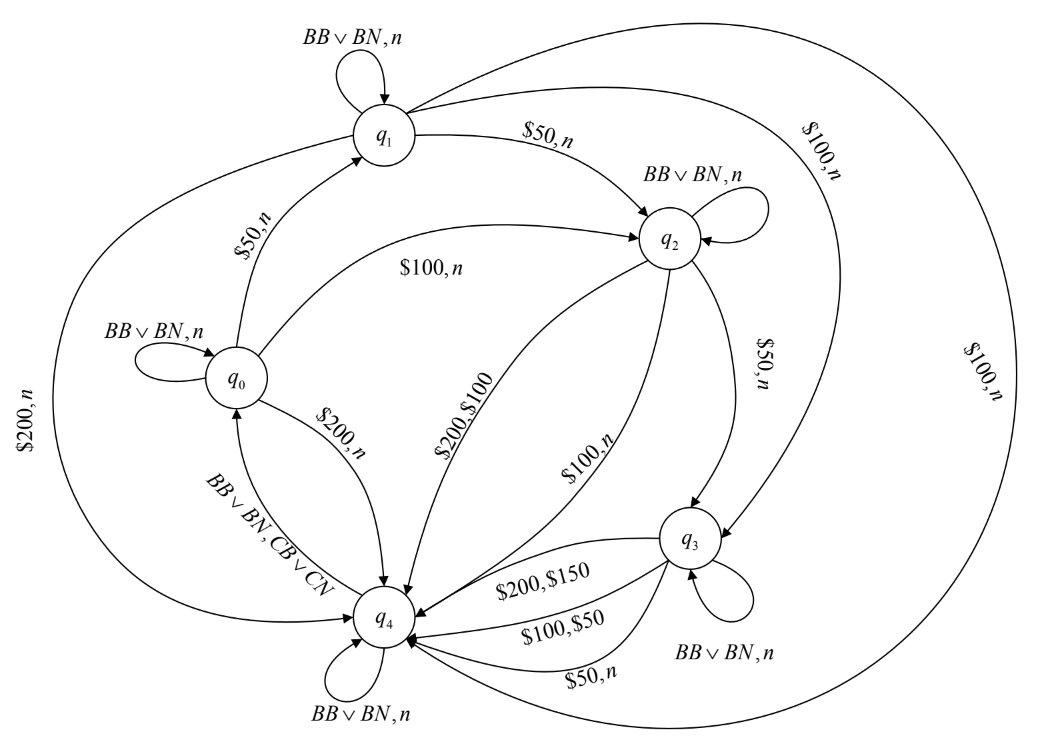
\includegraphics[width=120mm]{chapters/chapter4/figures/DTEmaquinaChocolatinas.png}
     \end{center}
     \textbf{\caption{DTE Para la máquina expendedora de chocolatinas.}}
\end{figure}

Para sistemas simples esta puede ser una tarea relativamente sencilla; sin embargo, cuando el sistema es complejo lo más probable es que su solución de tipo analítico sea imposible calcularla. Por esa razón, la alternativa plausible es encontrar una solución aproximada del modelo mediante técnicas de simulación. Aunque también es posible que sea imposible (principalmente por complejidad computacional), existe una mayor probabilidad de aproximar la solución con un nivel de error máximo permitido. Por este camino no se tiene la solución exacta o analítica pero si se puede encontrar una buena aproximación \cite{law1991simulationModeling}.\\

\section{SOLUCIÓN DEL MODELO MATEMÁTICO}\label{sec:SolModeloMatematico}
\subsection{Tipos de Soluciones}\label{subsec:TiposDeSoldeModMat}
Una vez se tiene el modelo, es necesario solucionarlo. Cuando se trata de un modelo matemático el objetivo es, generalmente, encontrar la solución al sistema de ecuaciones que modelan su comportamiento. De acuerdo con la Figura \arabic{chapter}—4 la solución del modelo matemático $\textfrak{MM}$ puede obtenerse o bien de forma analítica (también conocida como teórica o ideal) o bien a través de experimentación. Una de las formas más frecuentemente empleadas para encontrar la solución del modelo es mediante la técnica heurística llamada simulación.\\

\begin{figure}[H]
     \begin{center}
         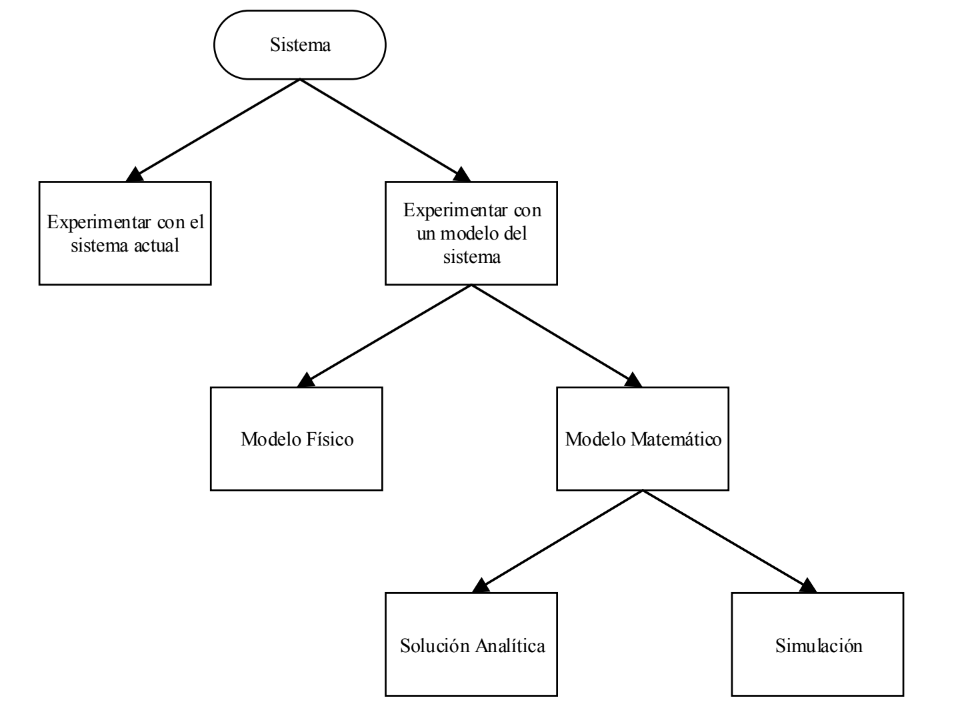
\includegraphics[width=120mm]{chapters/chapter4/figures/formasEstudioSistemaAverrilLaw.png}
     \end{center}
     \textbf{\caption{Posibles formas para estudiar un sistema (Tomada de \cite{law1991simulationModeling}).}}
\end{figure}

La simulación, por su lado, es para R.E. \textbf{Shannon}, \textit{” es el proceso de diseñar un \textbf{modelo} de un \textbf{sistema real} y llevar a término experiencias con él, con la \textbf{finalidad de comprender el comportamiento} del sistema o evaluar nuevas estrategias —dentro de los límites impuestos por un cierto criterio o un conjunto de ellos— para el funcionamiento del sistema”}. \textbf{Simular}, entonces, puede entenderse como sinónimo de \textbf{Imitar} con el fin de conocer el \textbf{comportamiento} del sistema para asumir algunas \textbf{decisiones} que afecten su actividad o estructura.\\

Existen varios paradigmas de simulación, entre los que se destacan tres: El \textbf{\textit{paradigma de dinámica de sistemas}}, el \textbf{\textit{paradigma de simulación de eventos discretos}} y el \textbf{\textit{paradigma de agentes artificiales}}. Una solución experimental del modelo matemático $\textfrak{MM}$ a través de simulación, típicamente, emplea los tres paradigmas antes mencionados.\\

\begin{table}[H]
\centering
\begin{tabular}{|p{2.2cm}|p{1.4cm}|p{1.4cm}|p{1.4cm}|p{0.1cm}|p{1.4cm}|p{1.4cm}|p{1.4cm}|}

                                  & \multicolumn{3}{c|}{\textbf{Ecuaciones Lineales}}                               & \multirow{}{}{} & \multicolumn{3}{c|}{\textbf{Ecuaciones no Lineales}}                            \\ \cline{1-4} \cline{6-8} 
\textbf{Ecuación}                 & \textbf{Una Ecuación} & \textbf{Varias Ecuaciones} & \textbf{Muchas Ecuaciones} &                   & \textbf{Una Ecuación} & \textbf{Varias Ecuaciones} & \textbf{Muchas Ecuaciones} \\ \cline{1-4} \cline{6-8} 
\textbf{Algebraica}               & Trivial               & Fácil                      & Casi Imposible             &                   & Muy Difícil           & Muy Difícil                & Imposible                  \\ \cline{1-4} \cline{6-8} 
\textbf{Diferenciales Ordinarias} & Fácil                 & Difícil                    & Casi                       &                   & Muy Difícil           & Imposible                  & Imposible                  \\ \cline{1-4} \cline{6-8} 
\textbf{Diferenciales Parciales}  & Difícil               & Casi                       & Imposible                  &                   & Imposible             & Imposible                  & Imposible                  \\ 
\end{tabular}
\caption{\textbf{Alcances y limitaciones de los modelos (Tomada de \cite{bertalanffy1968systemTheory}).}}
\label{tab:alcanLimitModelosVonBertalanffy}
\end{table}
\stepcounter{tableN}
\subsection{Limitaciones de los Modelos Matemáticos}\label{subsec:LimitdeModMat}
En este punto resulta interesante recordar los ya clásicos enunciados que se encuentran en \cite{bertalanffy1968systemTheory} y que se resumen en la Tabla ~\ref{tab:alcanLimitModelosVonBertalanffy}. En su disertación describe cómo los modelos matemáticos van desde los muy simples cuyas soluciones son relativamente triviales hasta los muy complejos en los cuales los sistemas de ecuaciones diferenciales parciales del modelo encontrado no tiene solución práctica.\\

En el marco del proyecto de estudio de un sistema complejo \textit{SC} esas conclusiones son importantes si se tiene en cuenta que los modelos matemáticos subyacentes al tipo de sistemas que se intenta comprender pueden tener decenas de ecuaciones diferenciales parciales que describen la dinámica de los estados del sistema en función del \textit{\textbf{espacio -- tiempo}}. En conclusión, las soluciones analíticas para este caso son imposibles de solucionar mediante una forma cerrada encontrada analíticamente.\\

Lo interesante es que a través de aproximaciones basados en estudios de simulación, \cite{law1991simulationModeling} han mostrado que ese tipo de inconvenientes pueden ser ignorados (al menos en parte con estudios serios de simulación).\\

\section{EL MODELO SAO}\label{sec:SAOModel}
De acuerdo con las clases de modelos que se deducen de la Figura \arabic{chapter}—4, SAO es un modelo matemático. Por cada elemento de la sigla existe un módulo: SAO (Sistema, Ambiente y Observatorio). Véase la Figura \arabic{chapter}—5.\\

\subsection{Módulos del Modelo}\label{subsec:ModulosdelModelo}
Aunque el \textit{\textbf{sistema}} es una entidad que puede ser estudiada de forma aislada, la verdad es que todos los sistemas se encuentran inmersos dentro de un \textit{\textbf{entorno}}. Por esa razón, al tiempo que se modela es sistema, es necesario también, incluir dentro del modelo, la representación del ambiente en el cual se desenvuelve ese sistema (puesto que se trata de determinar su comportamiento en ese ambiente particular).\\

\begin{figure}[H]
     \begin{center}
         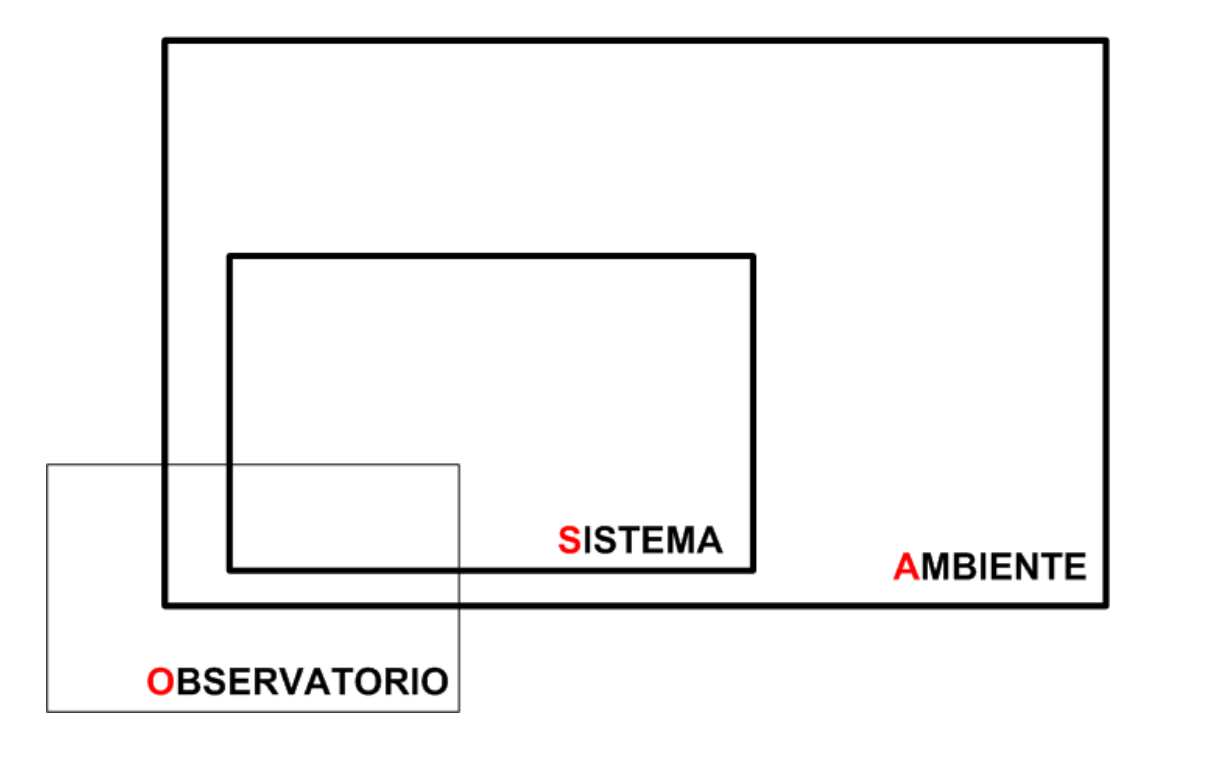
\includegraphics[width=90mm]{chapters/chapter4/figures/modeloSAO.png}
     \end{center}
     \textbf{\caption{Modelo SAO (Adaptado de \cite{trivino2012esthocasticModels})}}
\end{figure}

Con el fin de poder estudiarlo y caracterizarlo, se requiere un elemento más dentro de este esquema. Ese elemento fundamental dentro del propósito de realizar una simulación del sistema, es el \textit{\textbf{observatorio}}. El observatorio, como su nombre lo indica, tiene como finalidad medir o cuantificar u observar el desempeño de ese sistema dentro de ese ambiente. A todos los elemento que deben ser diseñados y, a la larga, simulados se les da el nombre genérico de Modelo SAO que se refiere a Sistema, Ambiente y Observador. Esa arquitectura se presenta de forma gráfica en la Figura \arabic{chapter}—5. Ese esquema es, precisamente, el seleccionado para construir el prototipo del sistema MIA.\\

\subsection{Especificación Matemática}\label{subsec:EspecifMatem}
Un segundo objeto matemático que caracteriza el ambiente es su \textit{\textbf{estado}}. Por ejemplo, en un sistema físico existen propiedades tales como la temperatura, la gravedad, el campo magnético, etc. Este tipo de objetos propios del ambiente se definen formalmente mediante las expresiones ~\ref{estadosConjDeAmbiente}.\\

\begin{equation}
\begin{matrix} $X \in \mathbb{R}^n$ \\ \ $X=(X_1,X_2,...,X_n)$ \end{matrix}
\label{estadosConjDeAmbiente}
\end{equation}

Cada una de las variables que conforman el Estado del sistema es, en sí misma, una función que depende del tiempo y del espacio como se escribe matemáticamente en la expresión ~\ref{estadoDeAmbiente1}.\\
\begin{equation}
\textit{\begin{matrix} $X_i:$ &  \mathbb{R}^m &$\to$&  \mathbb{R} \\ \ & $t$ & \to & $X_i = X_i(t)$ \end{matrix}}
\label{estadoDeAmbiente1}
\end{equation}

En sistemas de alta complejidad el estado del ambiente ~\ref{estadosConjDeAmbiente} es un vector aleatorio, lo cual supone la existencia de una estructura probabilística que lo rige, es decir, una función de densidad de probabilidad conjunta, como se escribe en la expresión ~\ref{funDensidadEstadoAmbiente1}.\\

\begin{equation}
\textit{$f_X(x)=f_{X_1,X_2,...,X_n}(x_1,x_2,...,x_n)$}
\label{funDensidadEstadoAmbiente1}
\end{equation}

Parámetros del Modelo son constantes que no cambiarán su valor durante una corrida de la simulación pero que, con el ánimo de poder realizar análisis de sensibilidad se dejan expresados no como valores específicos sino como letras que los representan. Formalmente se definen como en la expresión ~\ref{funParametros}\\

\begin{equation}
\begin{matrix} $\xi \in \mathbb{R}^q$ \\ \ $\xi=(\xi_1,\xi_2,...,\xi_q)$ \end{matrix}
\label{funParametros}
\end{equation}

Por último, los comportamientos, leyes o características, definidas formalmente mediante la expresión ( \ref{comportamientosEq}), son propiedades de sistemas que pretende con el estudio estimar, encontrar o corroborar. Ellos son la razón de ser de la simulación puesto que son conductas que muchas veces ni siquiera se sabe que existen pero son una realidad la gran mayoría de las veces ocultas. La ley de gravedad en el universo físico es una de ellas. Están ahí y afectan a los objetos que actúan en ese contexto pero normalmente no se tiene conciencia de ellas.\\

\begin{figure}[H]
     \begin{center}
         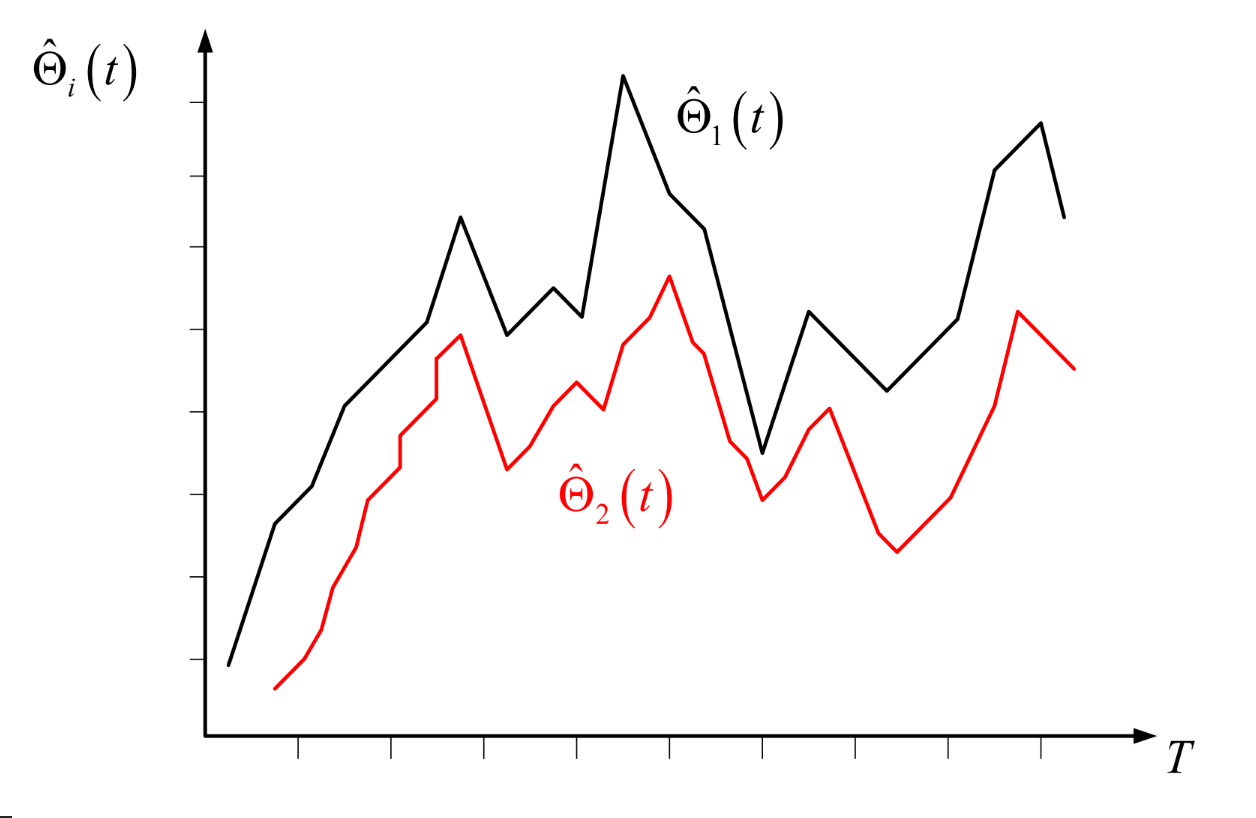
\includegraphics[width=90mm]{chapters/chapter4/figures/leyesObservatorio.png}
     \end{center}
     \textbf{\caption{Dos leyes hipotéticas encontradas por el Observatorio con base en la simulación.}}
\end{figure}

Una vez identificadas el investigador puede usarla para, por ejemplo, mejorar algún índice (en el caso de sistemas con participación humana) de calidad de vida o, por qué no, concluir que una mejora en tal índice es imposible.\\

\begin{equation}
\begin{matrix} $\Theta \in \mathbb{R}^p$ \\ \ $\Theta=(\Theta_1,\Theta_2,...,\Theta_p)$ \end{matrix}
\label{comportamientosEq}
\end{equation}

Las leyes dadas en la expresión ( \ref{comportamientosEq} ) junto con los parámetros dados en la expresión ( ~\ref{funParametros} ) van a permitir definir estrategias y políticas sobre el sistema puesto que a través de la variación de los parámetros se podrá deducir el impacto que ese cambio o variación ejerce sobre el comportamiento base del análisis de sensibilidad; puesto que como se observa de la expresión ( ~\ref{LeyesyParam}) las leyes también dependen de los parámetros. Por eso es posible (y deseable e incluso necesario) realizar estudios de análisis de sensibilidad.\\

\begin{equation}
\textit{\begin{matrix} $\Theta_i:$ & \mathbb{R}^{m+n+q+1} &$\to$& \mathbb{R} \\ \ & $t,x,\xi,F_X$ & \to & $\Theta_i = \Theta_i(t,x,\xi,F_X)$ \end{matrix}}
\label{LeyesyParam}
\end{equation}

En este punto es donde se evidencia el rol tan importante del observatorio en el modelo SAO. Ese módulo del software (que en ocasiones incluye también hardware) tiene que emplear el esquema de la simulación para estimar o aproximar una o todas las leyes supuestas en la expresión (\ref{comportamientosEq}). Es decir, construir las tablas que aproximan la dinámica subyacente en la ley (por ejemplo un indicador del sistema MIA). Gráficamente, la Figura \arabic{chapter}—6, muestra lo que arrojaría el Observatorio con base en los mecanismos de simulación que tiene el prototipo.\\

\begin{figure}[H]
     \begin{center}
         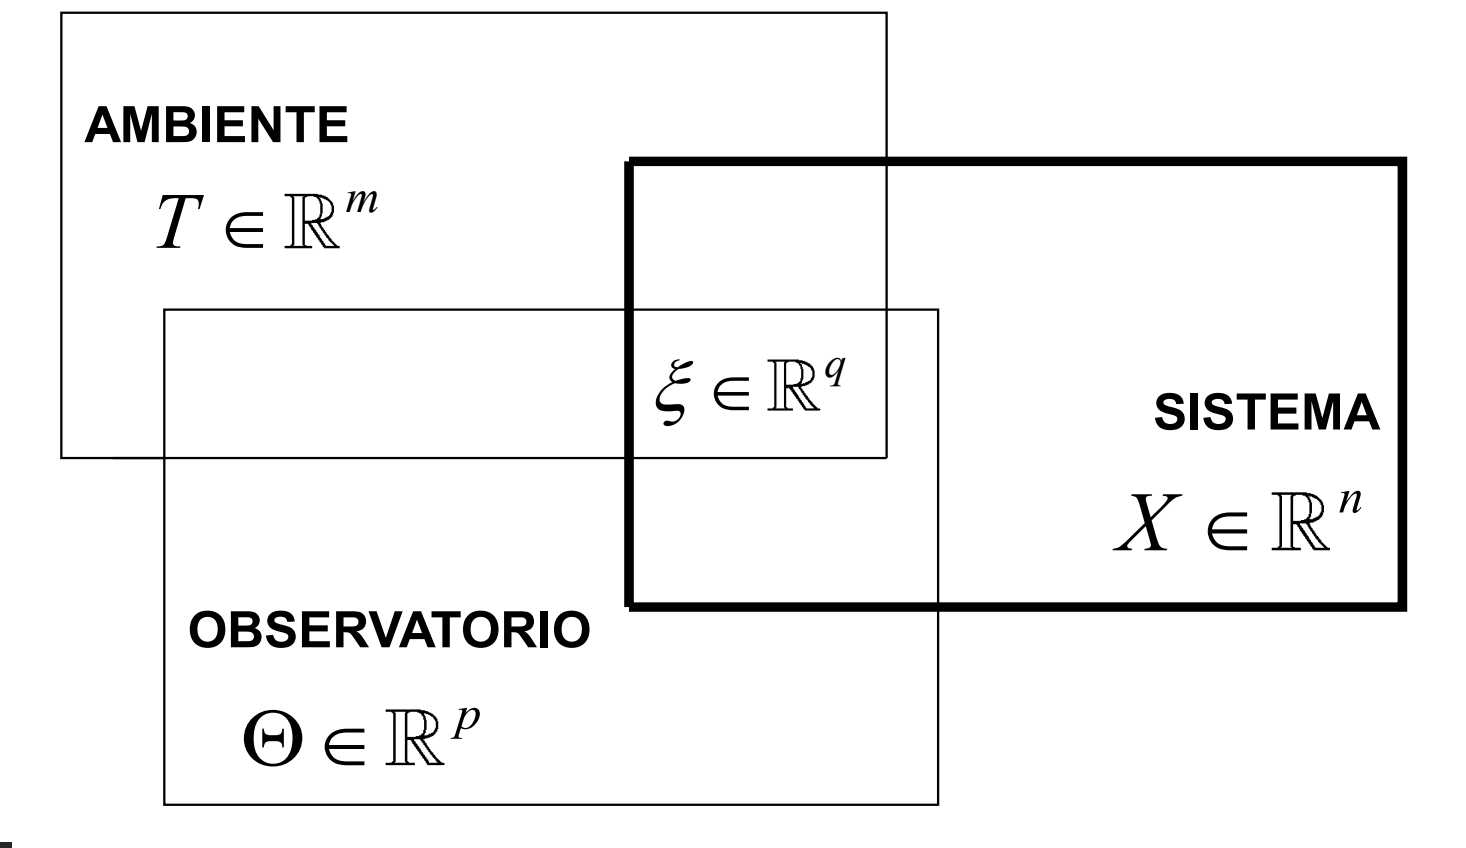
\includegraphics[width=90mm]{chapters/chapter4/figures/modeloMatSAO.png}
     \end{center}
     \textbf{\caption{Representación gráfica y matemática del modelo SAO.}}
\end{figure}

Un análisis intuitivo de la Figura \arabic{chapter}—6 indica que el vector de leyes ( \ref{comportamientosEq}) es un proceso estocástico multivariado cuya estructura probabilística, escrita formalmente en la expresión (\ref{ProbvectorLeyes}), no se conoce pero que se puede inferir (al menos su características y propiedades básicas) a partir de los datos arrojados por el simulador. Ese análisis realizado, por ejemplo, mediante series de tiempo multivariadas. Con seguridad, para los resultados supuestos de la Figura \arabic{chapter}—6, demostrarán lo que es evidente en la mencionada figura: que las leyes $\Theta_1$ y $\Theta_2$ tienen un alto grado de correlación o similitud.\\

\begin{equation}
\textit{$f_\Theta(\omega)=f_{\Theta_1,\Theta_2,...,\Theta_p}(\omega_1,\omega_2,...,\omega_p)$}
\label{ProbvectorLeyes}
\end{equation}

El modelo SAO, en resumen, se puede describir en breve como en la Figura \arabic{chapter}—7.\\

\textbf{Definición \arabic{chapter}-\arabic{definitionN}: Modelo matemático $\textfrak{MM}_{SAO}$ de la configuración SAO }\\
\stepcounter{definitionN}

El modelo matemático para una configuración SAO, $\textfrak{MM}_{SAO}$ es un objeto matemático definido mediante la tupla $\textfrak{MM}_{SAO}=(M_S,M_\Delta,M_O,I)$ en la cual:\\

\begin{enumerate}
    \item \textit{$M_{\mathbb{S}}$} es una maquina de estados finitos que modela el sistema $\mathbb{S}$.
    \item \textit{$M_\Delta$} es una máquina de estados finitos que modela el ambiente $\Delta$.
    \item \textit{$M_O$} es una máquina de estados finitos que modela el observatorio O.
    \item \textit{$I= \left\lbrace \ell_{i,j} \right\rbrace_{i,j \in \left\lbrace S, \Delta, O \right\rbrace}$} con $\ell_{i,j} = \left\lbrace \ell_{i,j}^k \right\rbrace_{k=1}^{l_{i,j}}$ es el conjunto de $l_{i,j}$ interfaces de comunicación entre el módulo $i$ y el módulo $j$ $(i \neq j)$. En sí misma, cada interfaz $\ell_{i,j}^k$ es (en general, mas no necesariamente en particular) una máquina de estados finitos.
\end{enumerate}


\section{SIMULACIÓN DE EVENTOS DISCRETOS}\label{sec:SimulEventDiscret}

Históricamente los investigadores en Simulación se han enfocado en los distintos componentes del comportamiento (optimización, aprendizaje, razonamiento, visión,....), de forma aislada. Eso ha causado que, en ciertas circunstancias (especialmente cuando se simulan sistemas complejos) los resultados no hayan sido del todo satisfactorios. En la actualidad, se sugiere \cite{trivino2012esthocasticModels} que \textbf{\textit{la Simulación, es producto de la interacción entre una comunidad de agentes (SS) y su entorno.}} Entonces, comportamientos complejos, que no han sido modelados, emergen de la interacción de varios comportamientos simples como los agentes artificiales; sin embargo, el marco clásico de la simulación de sistemas complejos sigue aún muy vigente.\\

Por consiguiente, en este capítulo se exponen los principales elementos de una simulación tradicional y se deja para otro capítulo el desarrollo con más detalle del paradigma de agentes. Así, simulación clásica y simulación basada en agentes no son conceptos disyuntos ni incompatibles, al contrario, el paradigma de agentes hace más robustos los modelos de simulación.\\

\textbf{Definición \arabic{chapter}-\arabic{definitionN}: Evento }\\
\stepcounter{definitionN}

Un evento es un acontecimiento que ocurre en algún instante en el Tiempo-Espacio (de la simulación) y que cambia el estado del sistema. La Figura \arabic{chapter}—8 representa esa visión.\\

Cada vez que ocurre un evento se disparan un conjunto de acciones que tienden a actualizar el valor de las variables de estado. En simulación clásica, la ocurrencia de un evento dispara automáticamente un procedimiento asociado específicamente con el tipo de evento que está ocurriendo. Por su lado, bajo el paradigma de agentes (discutido en un capítulo aparte de este pero estrechamente relacionado) el evento activará a la comunidad de agentes asociados con ese evento. Los agentes percibirán su entorno y, al unísono, ejecutarán sus acciones que afectarán el estado del ambiente y el de ellos mismos por supuesto (véase el Ejemplo \arabic{chapter}—5 como ilustración).\\

\begin{figure}[H]
     \begin{center}
         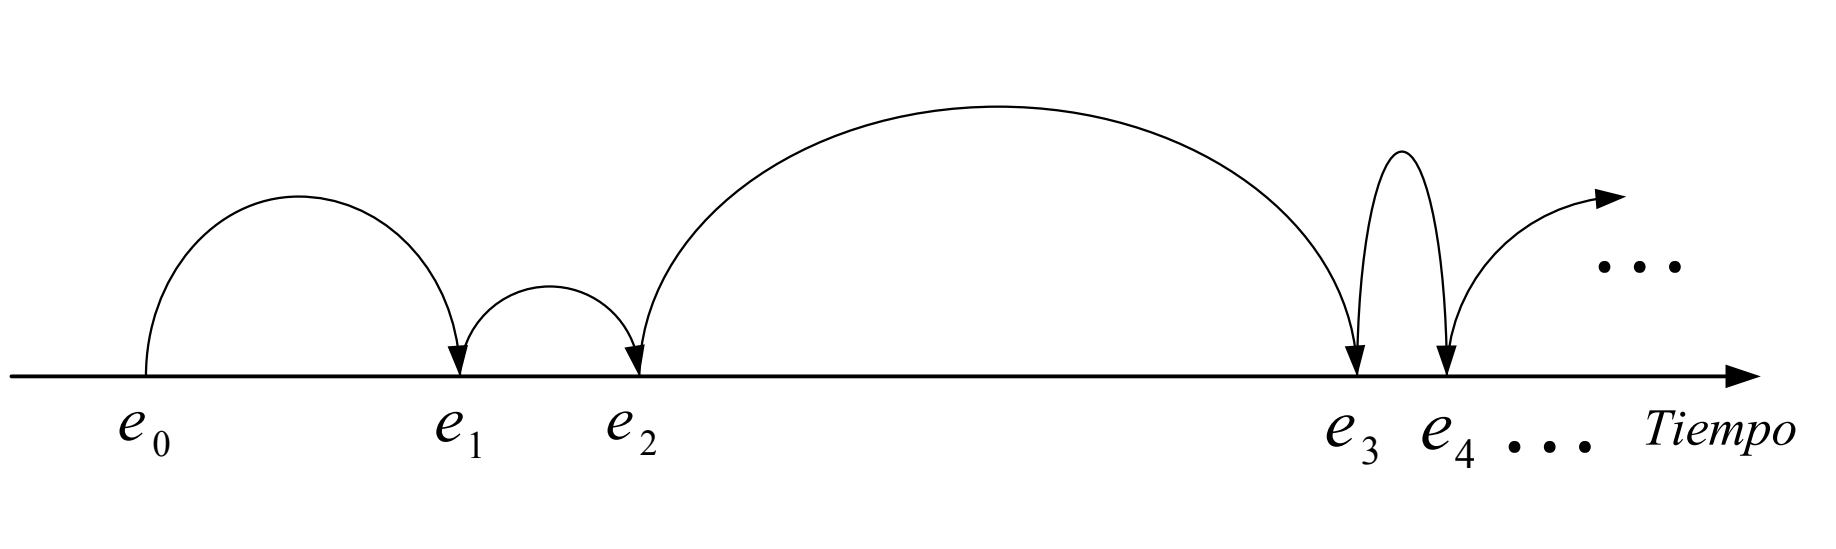
\includegraphics[width=90mm]{chapters/chapter4/figures/relacTiempoEvento.png}
     \end{center}
     \textbf{\caption{Relación entre tiempo y eventos.}}
\end{figure}


\subsection{Arquitectura de la Aplicación }\label{subsec:ArquitDeLaApp}

Un esquema general para abordar cualquier problema de simulación se puede esquematizar implementando el siguiente conjunto de algoritmos que parten de la idea de eventos discretos. El primer algoritmo importante es inicialización, cuya estructura se muestra en el Algoritmo \arabic{chapter}—1. Su propósito es colocar los niveles iniciales de todo el conjunto de variables que participan en la simulación.\\

\begin{center}
\textit{
\raggedright
PROCEDIMIENTO INICIALIZACIÓN($\langle$ Argumentos$\rangle$)\\
\quad INICIO\\
\quad \quad $T \gets$ $\langle$ValoresInicialesTiempoEspacio$\rangle$;\\
\quad \quad $X \gets$ $\langle$ValoresInicialesEstudioSistema$\rangle$;\\
\quad \quad $\theta \gets$ $\langle$ValoresInicialesCaracteristicasSistema$\rangle$;\\
\quad \quad $\xi \gets$ $\langle$ValoresInicialesParametrosSistema$\rangle$;\\
\quad \quad $L \gets$ $\langle$ValoresInicialesListaEventos$\rangle$; // Se emplea función percentil\\
\quad FIN\_PROCEDIMIENTO\_INICIALIZACIÓN\\}

\textbf{Algoritmo \arabic{chapter}-\arabic{algorithmN}: Procedimiento de inicialización.}\\
\end{center}\\
\stepcounter{algorithmN}

Otra función importante dentro del esquema general del simulador lo constituye el manejo del tiempo espacio. En un sentido general es un procedimiento cuya finalidad es manejar el reloj de la simulación. Su estructura lógica se muestra en el Algoritmo \arabic{chapter}—2.\\

\begin{center}
\textit{
\raggedright
$\mathbb{N}$ FUNCION ManejoTiempoEspacio($\langle$Argumentos$\rangle$)\\
\quad INICIO\\
\quad \quad $k^* \gets \{ k | L[k] == min_\gamma\{ L[\gamma]\}\}$; // Próximo evento\\
\quad \quad $T \gets L[k^*]$; // Actualizar el Tiempo Espacio: ''Reloj''\\
\quad \quad RETORNAR($k^*$);\\
\quad FIN\_FUNCION\_ManejoTiempoEspacio\\ }

\textbf{Algoritmo \arabic{chapter}-\arabic{algorithmN}: Función para manejar el tiempo y el espacio del simulador.}\\
\end{center}\\

\stepcounter{algorithmN}

De forma similar, por cada tipo de evento que presente el sistema a simular, debe incluirse una función que se encargue de actualizar adecuadamente el conjunto de variables de estado y de características del sistema. Esa labor la desarrolla el Algoritmo \arabic{chapter}—3.\\

\begin{center}
\textit{
\raggedright
$\mathbb{R}$ FUNCIÓN EVENTO\_$i$($\langle$Argumentos$\rangle$)\\
\quad INICIO\\
\quad \quad $X \gets$ $\langle$ActualizarEstudioSistema$\rangle$;\\
\quad \quad $\theta \gets$ $\langle$ActualizarCalculoCaracteristicas$\rangle$;\\
\quad \quad $L \gets$ $\langle$ActualizarListaEventos$\rangle$; // Usar Funciones Percentiles\\
\quad FIN\_FUNCIÓN\_EVENTO\_$i$\\ 
}
\textbf{Algoritmo \arabic{chapter}-\arabic{algorithmN}: Estructura general del evento i.}\\
\end{center}\\

\stepcounter{algorithmN}

La aplicación práctica del teorema fundamental de la simulación, presentado en la sección anterior se lleva a cabo en el Algoritmo \arabic{chapter}—4.\\

El Algoritmo \arabic{chapter}—6 tiene la misión de dirigir el llamado de todas las funciones y procedimientos descritas anteriormente. Esa ejecución debe hacerse de manera ordenada y sistemática y a su debido momento. Esa es la labor de este procedimiento principal, que se describe en el Algoritmo \arabic{chapter}—6.

\begin{center}
\textit{
\raggedright
$\mathbb{R}$ FUNCIÓN PercentilContinuaGeneral($\langle$ParámetrosPoblacionales$\rangle$)\\
\quad INICIO\\
\quad \quad $u \gets$ Aleatorio($\bullet$);\\
\quad \quad $x \gets$ $F_x^{-1}(u)$;\\
\quad \quad RETORNAR($x$);\\
\quad FIN\_FUNCIÓN\_PercentilContinuaGeneral\\ 
}
\textbf{Algoritmo \arabic{chapter}-\arabic{algorithmN}: Implementación de una función percentil.}\\
\end{center}\\

\stepcounter{algorithmN}

Finalmente se debe ejecutar un procedimiento que muestre los reportes de las estadísticas finales que muestre los resultados de la simulación. Esta tarea la realiza el Algoritmo \arabic{chapter}—5.\\

\begin{center}
\textit{
\raggedright
 PROCEDIMIENTO GeneradorReporte($\langle$Argumentos$\rangle$)\\
\quad INICIO\\
\quad \quad $\theta \gets$ $\langle$CalculoFinalDeCaracterísticas$\rangle$;\\
\quad \quad ESCRIBIR($\theta$);\\
\quad FIN\_PROCEDIMIENTO\_GeneradorReporte\\ 
}
\textbf{Algoritmo \arabic{chapter}-\arabic{algorithmN}: Procedimiento de reporte de la simulacíon.}\\
\end{center}\\

\stepcounter{algorithmN}


\subsection{Metodología de la Simulación}\label{subsec:MetodDeLaSimul}

La metodología de la simulación, como es de esperarse, está fuertemente inspirada en el método científico. Sus pasos o etapas están estrechamente relacionados con ese método. La Figura \arabic{chapter}—9 presenta, en forma de diagrama de flujo las diez etapas que la componen y que fueron adoptadas en la construcción del sistema MIA. Un mayor detalle en la descripción de cada uno de los pasos presentados se puede encontrar en \cite{law1991simulationModeling} y en \cite{trivino2010complexSystems}. Es necesario seguir con extremo rigor estos pasos y sus recomendaciones.\\

En síntesis, y en explicación de la Figura \arabic{chapter}—9, los pasos de la metodología consisten en:\\

\textbf{\textit{\underline{Etapa \# 01:} Formulación del problema y el plan de estudio.}}\\

El problema de interés se fija y se formaliza. Esta labor debe ser realizada por el director del área. Usualmente se llevan a cabo una o más reuniones con esta finalidad en la cual deben asistir el director del proyecto, el analista de simulación, y expertos en la materia: En esas reuniones se deberían discutir los siguientes temas:\\

\begin{enumerate}
    \item Los objetivos generales del estudio.
    \item Preguntas específicas que serán resueltas por el estudio.
    \item Las medidas de desempeño que se utilizarán para evaluar la eficacia de diferentes
configuraciones del sistema.
    \item Alcance del modelo.
    \item Configuraciones y escenarios del sistema a ser modelados.
    \item Herramientas de cómputo, específicamente Hardware y Software que se va utilizar.
    \item Periodo de tiempo para el estudio y los recursos necesarios.
\end{enumerate}

\begin{center}
\textit{
\raggedright
$\mathbb{N}$ FUNCIÓN SimuladorPrincipal($\langle$Argumentos$\rangle$)\\
\quad INICIO\\
\quad \quad CodError$ \gets$ $0$;\\
\quad \quad Inicialización($\langle$Argumentos$\rangle$);\\
\quad \quad MIENTRAS($\langle$NoHayaCondiciónTerminación$\rangle$,$\land$,CodError==$0$) HACER\\
\quad \quad \quad INICIO\\
\quad \quad \quad \quad i $\gets$ ManejoTiempoEspacio($\langle$Argumentos$\rangle$);\\
\quad \quad \quad \quad SELECCIONAR(i) DE\\
\quad \quad \quad \quad \quad INICIO\\
\quad \quad \quad \quad \quad \quad CASO 1: Evento\_1($\langle$Argumentos$\rangle$);\\
\quad \quad \quad \quad \quad \quad CASO 2: Evento\_2($\langle$Argumentos$\rangle$);\\
\quad \quad \quad \quad \quad \quad \quad \quad \quad $\vdots$ \\
\quad \quad \quad \quad \quad \quad CASO i: Evento\_i($\langle$Argumentos$\rangle$);\\
\quad \quad \quad \quad \quad \quad \quad \quad \quad $\vdots$ \\
\quad \quad \quad \quad \quad \quad CASO m: Evento\_m($\langle$Argumentos$\rangle$);\\
\quad \quad \quad \quad \quad FIN\_SELECCIONAR\\
\quad \quad \quad FIN\_MIENTRAS\\
\quad \quad  GeneradorReporte($\langle$Argumentos$\rangle$);\\
\quad FIN\_SimuladorPrincipal\\ 
}
\textbf{Algoritmo \arabic{chapter}-\arabic{algorithmN}: Estructura general de un simulador para sistemas dinámicos.}\\
\end{center}

\stepcounter{algorithmN}


\begin{figure}[H]
     \begin{center}
         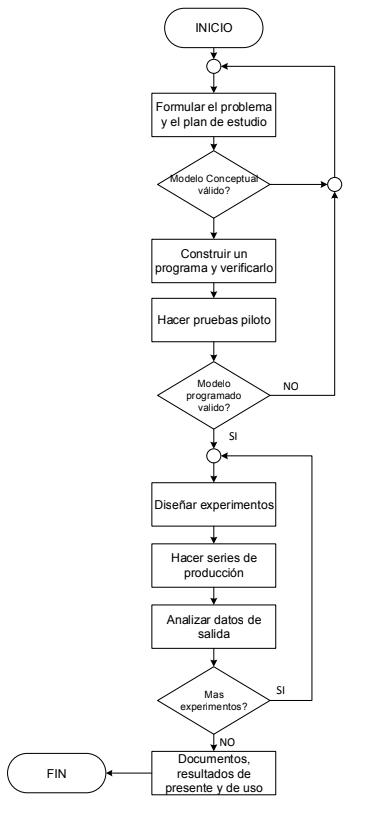
\includegraphics[width=6cm]{chapters/chapter4/figures/metodDeSimulacion.png}
     \end{center}
     \textbf{\caption{Metodología de la Simulación (Adaptada de \cite{law1991simulationModeling})}}
\end{figure}

\textbf{\textit{\underline{Etapa \# 02:} Recolección de datos y definición del modelo.}}\\

Recopilar información sobre el diseño del sistema y los procedimientos de operación. Verificar la calidad de la información puesto que, en ciertas ocasiones cuando se trabaja con información que tienen algunas personas esa información puede ser inexacta.\\

Luego, recolectar datos (si ello es posible) para estimación de parámetros específicos del modelo y las distribuciones de probabilidad de entrada. Delinear esta información anterior y los datos en un ''documento de supuestos''. Cuál es el modelo conceptual. Así mismo, de ser posible, recolectar datos sobre el rendimiento del sistema existente (Para fines de validación en el Paso 6). El nivel de detalle del modelo debe depender de lo siguiente:\\

\begin{enumerate}
    \item Objetivos del proyecto
    \item Medidas de desempeño
    \item Problemas de Credibilidad
    \item Restricciones de ordenador
    \item Las opiniones de los PYME
    \item Las limitaciones de tiempo y dinero
\end{enumerate}

Al ser un modelo, no tiene que haber una correspondencia uno a uno entre cada elemento del modelo y el elemento correspondiente del sistema. Por ello es necesario identificar los más relevantes.\\

\textbf{\textit{\underline{Etapa \# 03:} ¿Es válido el modelo conceptual?}}\\

Realizar un recorrido del modelo conceptual utilizando el documento de supuestos antes de una audiencia con los gerentes y los analistas.\\

\textbf{\textit{\underline{Etapa \# 04:} Construir un prototipo de software y verificarlo.}}\\

Programar el modelo en un lenguaje de programación (por ejemplo, C, JAVA, PHYTON), o en el software de simulación (por ejemplo, un FrameWork de agentes). Emplear un lenguaje de alto nivel tiene un beneficio claro puesto que se conoce, tiene un costo de compra bajo, y puede resultar en un tiempo de ejecución del modelo más pequeño. El uso de software de simulación reduce el tiempo de programación y los resultados en un costo del proyecto menor pero se restringe a las limitaciones y posibilidades de la herramienta.\\

\textbf{\textit{\underline{Etapa \# 05:} Hacer pruebas piloto.}}\\

Esta etapa permite la validación necesaria en el Paso 6 de esta metodología.\\

\textbf{\textit{\underline{Etapa \# 06:} ¿El modelo programado es válido?}}\\

Si hay un sistema real, a continuación, comparar el modelo (implementado) y el sistema. Realizar pruebas de sensibilidad.\\

\textbf{\textit{\underline{Etapa \# 07:} Diseño de experimentos.}}\\

Para cada uno de los escenarios de interés determinar el número de corridas, el periodo de calentamiento necesario.\\

\textbf{\textit{\underline{Etapa \# 08:} Ejecutar las corridas definitivas.}}\\

Estas corridas son necesarias para la realización del paso 9 de ésta metodología el cual tiene como propósito obtener los resultados definitivos.\\

\textbf{\textit{\underline{Etapa \# 09:} Análisis de la información de salida.}}\\

Usualmente se acompaña de la aplicación de métodos estadísticos que le dan formalidad al análisis. El propósito de esta etapa es obtener el conjunto de datos resumidos en tablas que describen las dinámicas de las leyes que se desea estimar. Cada dato debe haber sido calculado con un error máximo permitido y una significancia determinada por el investigador. También en esta fase se pueden comparar los diferentes escenarios simulados.\\

\textbf{\textit{\underline{Etapa \# 10:} Informe y resultados.}}\\

Elaboración del documento final en el cual se plasman los resultados más importantes que muestran
los estudios de simulación realizados. Frecuentemente, estos datos son enviados a un experto quien
deberá tomar decisiones que afecten al sistema basado en lo que el informe le está comunicando.\\

\section{RESUMEN Y PANORAMA HISTÓRICO }\label{sec:ResumenyPanHisoric}
\section{EJERCICIOS}\label{sec:EjerciciosModySimul}

\begin{enumerate}
    \item Analizar, diseñar e implementar (en algún lenguaje de programación, se sugiere Python o Java), una aplicación que permita simular, es decir que cuente con las funcionalidades descritas en la sección \ref{subsec:ArquitDeLaApp}, para cualquier sistema $\mathbb{S}$ que pueda abstraerse a través del modelo matemático SAO propuesto en la Definición \arabic{chapter}—11.\\
    
    \item Para el Ejemplo \arabic{chapter}—5, aplique la Definición 1—5 para proponer un ambiente para este sistema y la Definición \arabic{chapter}—10 para obtener su modelo matemático.\\
    
    \item Emplear el Ejemplo \arabic{chapter}—5, el Ejemplo \arabic{chapter}—8 y los resultados de los Ejercicios 2 y 3 como primer escenario de prueba para la aplicación construida en el Ejercicio 1.\\
    
    \item Proponer otros dos sistemas $\mathbb{S}_1$ y $\mathbb{S}_2$ , obtener sus respectivos modelos matemáticos $\textfrak{MM }_{SAO}^1$ y $\textfrak{MM }_{SAO}^2$, y simularlos en la aplicación construida en el Ejercicio 1.\\
    
    \item Para el sistema dado en el Ejemplo \arabic{chapter}—4
    \begin{enumerate}
        \item Aplicar la Definición \arabic{chapter}—8 para encontrar su modelo matemático.
        \item Aplicar la Definición \arabic{chapter}—11 para determinar su modelo matemático SAO.
    \end{enumerate}
\end{enumerate}

%\chapter{TEOREMA FUNDAMENTAL DE LA SIMULACIÓN}
%\chapter{ARQUITECTURA GENERAL DE UN SIMULADOR DE SISTEMAS COMPLEJOS}
%\chapter{FUNCIONES PERCENTILES,TRUNCADAS Y CONTAMINADAS CONJUNTAS}
%\chapter{MODELOS DE MOVILIDAD}
%\chapter{LENGUAJES DE PROGRAMACIÓN PARA SIMULACIÓN DE REDES}
%\chapter{DISTRIBUCIÓN LAMBDA GENERALIZADA}
